\documentclass[11pt,a4paper]{article}
\usepackage[margin=25mm]{geometry}
\usepackage[T1]{fontenc}
\usepackage{lmodern}
\usepackage{amsmath,amssymb,booktabs,array,longtable,graphicx,tabularx,multirow}
\usepackage{microtype}
\usepackage{placeins}
\usepackage{hyperref}
\graphicspath{{figures/}}
\newcommand{\Rtwentynine}{R29}
\newcommand{\Othirtytwo}{O32$-$71}
\newcommand{\med}{\operatorname{median}}
\newcommand{\dd}{\mathrm{d}}
\newcommand{\suppsec}[1]{Supplement #1}
\newcolumntype{Y}{>{\raggedright\arraybackslash}X}
\setlength{\emergencystretch}{3em}
\hypersetup{hidelinks,pdftitle={Recalibration Can Mask Measured Sensitivity to Receiver-Coordinate Errors in RSSI Localization},pdfauthor={Ananta Ranjan and Vijay Kumar Jha}}
\title{Recalibration Can Mask Measured Sensitivity to Receiver-Coordinate Errors in RSSI Localization}
\author{Ananta Ranjan\thanks{Correspondence: phdcs10011.20@bitmesra.ac.in} \and Vijay Kumar Jha\thanks{Email: \href{mailto:vkjha@bitmesra.ac.in}{vkjha@bitmesra.ac.in}}}
\date{Department of Computer Science and Engineering\\Birla Institute of Technology, Mesra, Ranchi 835215, Jharkhand, India}
\begin{document}
\maketitle
\begin{abstract}
Recalibration can suppress the measured median-error response to receiver-coordinate corruption without correcting the coordinates. We investigate calibration, receiver participation, and spatial error structure in four received-signal-strength-indicator (RSSI) localization pipelines on a public LoRaWAN corpus with recovered and catalogue-derived coordinate configurations. A paired intervention holds corrupted coordinates, receptions, and evaluation messages fixed while refitting or freezing receiver-specific intercepts. Across 32 direction fields with the two highest-participation receivers displaced by 5 km, refitted weighted-centroid localization (WCL) median error changes by 1.5\% and -1.8\% on the two configurations, compared with 99.8\% and 50.2\% with frozen intercepts. Paired median-error benefits are positive in all 32 two-receiver cases per configuration, but refitting is harmful in four of 32 one-receiver cases on the catalogue-derived configuration. Weight and affected-message diagnostics connect these responses to calibration-induced reweighting, not solely to unaffected messages. Cross-window controls trace a geographically concentrated transition to receiver identity and selected support; a failed rotation transfer is interpreted through reference geometry and pivot-induced translation. These finite-corpus findings establish calibration-dependent measured sensitivity, not map validity or universal protection. Coordinate-robustness assessments must specify the injected error, participating receivers, reference geometry, and calibration state.
\end{abstract}
\noindent\textbf{Keywords:} RSSI localization; receiver-coordinate uncertainty; calibration; LoRaWAN; receiver participation; reproducibility

\section{Introduction}\label{sec:intro}
The same receiver-coordinate corruption can produce substantially different changes in median localization error depending on whether the evaluation permits recalibration. A localization system can therefore maintain a nearly unchanged aggregate error even when its receiver coordinates have been displaced severely. Stable aggregate localization error is not, by itself, evidence that those coordinates are accurate or that individual position estimates remain unchanged. This distinction matters when receiver maps come from catalogues, installation records, global navigation satellite system measurements, or earlier self-localization.

Refitted and frozen calibration answer different operational questions. Refitting evaluates a pipeline with an opportunity to adapt its radio parameters to the supplied map; freezing evaluates the coordinate change while retaining the previous radio calibration. Both conditions yield genuine performance measurements under their respective assumptions. Here, \emph{masking} denotes suppression of the aggregate error response by adaptation, not correction of the physical coordinates or fictitious accuracy. A robustness conclusion must specify which calibration opportunity was available.

Anchor-position uncertainty is already addressed by uncertainty-aware estimators and theoretical bounds \cite{ref1,ref2,ref3,ref4,ref5,ref6,ref7,ref8,ref9,ref10,ref11,ref12,ref13,ref14}. Our principal question is how much the calibration state itself changes measured coordinate sensitivity when the corruption, observations, receiver selection and evaluation identities are held fixed. We investigate that question through a matched weighted-centroid localization (WCL) intervention, supported by a broader four-pipeline study of corruption load, receiver participation and reference-frame construction on the public Antwerp LoRaWAN corpus.

The principal finding is a large, but conditional, calibration-state effect. With the two highest-participation receivers displaced by 5~km, the across-field WCL median-error changes are $+1.5\%$ and $-1.8\%$ with refitting, compared with $+99.8\%$ and $+50.2\%$ with frozen intercepts on recovered R29 and catalogue-derived O32$-$71. All 32 two-receiver paired contrasts favor refitting in each configuration. Four one-receiver O32$-$71 fields instead favor freezing. Quantified intercept, weight and affected-message diagnostics explain how recalibration changes the response while showing that downweighting need not improve accuracy in every field.

Two complementary findings delimit the interpretation. In the O33-substituted receiver-window control, BS10 and the same 335 messages track the larger of the two adjacent error rises across $k=5$--7 as the receiver's rank moves from seven to six for WCL, ABS and DIFF; Min-Max is an exception. This is an identity-traced association with selected support, not an isolated effect of support loss, and the affected messages are geographically concentrated. Separately, a rotation ordering fails to transfer between native coordinate configurations. An exact change-of-pivot identity and the full sampled control distribution clarify how reference geometry and pivot choice change the prescribed displacement field.

The contribution is a controlled quantification of calibration-dependent measured sensitivity, with numerical diagnostics and counterexamples, together with participation and geometric analyses that specify further limits on robustness interpretation. The four-pipeline load surface supplies broader finite-design context. All comparisons remain conditional on the recorded campaign and the named reference configurations: R29 is a fixed historical assignment with incomplete selection provenance, and catalogue-derived controls do not certify physical coordinate accuracy. Exact inputs, implementation rules and retained results accompany the study.

\section{Related Work}\label{sec:related}
Uncertain-anchor localization has been addressed using semidefinite and second-order-cone relaxations \cite{ref1,ref2}, joint maximum-likelihood estimation \cite{ref3}, RSS-difference formulations with unknown transmit power \cite{ref4}, and geometric analyses of Fisher information and attainable accuracy \cite{ref5,ref13}. These studies establish the dependence of localization accuracy on topology and anchor uncertainty.

Practical RSS approaches include bias-compensated pseudo-linear estimation, iterative self-localization, semidefinite methods for Gaussian or bounded anchor uncertainty, and joint learning under impulsive noise \cite{ref6,ref7,ref8,ref9,ref11}. Li et al. validate uncertainty-aware cooperative RSS localization on a 50-node Bluetooth Low Energy deployment with accurate positional reference measurements \cite{ref10}. Gur and Sabach study large-scale sensor-network localization under a truncated multivariate-normal anchor-uncertainty model \cite{ref12}. Hybrid RSS/time-of-arrival analysis also treats inaccurate anchors under stratified propagation \cite{ref14}. These methods principally develop estimators or bounds under specified uncertainty models. The present experiment holds four implemented pipelines fixed and changes the perturbation and calibration conditions under which robustness is measured.

Reference-frame interpretation and receiver selection provide two further precedents. Ash and Moses distinguish relative position error and transformation components in self-localization \cite{ref16}. This geometric perspective motivates explicit translation, rotation and scale controls and the change-of-pivot analysis used here. Sensor-selection studies consider the incremental value of a sensor under resource and error constraints, including a knapsack formulation whose stated error criterion is nonlinear and submodular \cite{ref17}, and channel-knowledge-based selection \cite{ref18}. Here, selected receivers arise from recorded RSSI-ranked participation rather than an optimized deployment. We examine corruption of those existing receiver sets and test the relationship between identity, selected support and observed localization damage.

Unknown-parameter treatment provides a closer comparison. Li et al.~\cite{ref10} jointly estimate target locations, transmit powers and the path-loss exponent while accounting for anchor-location uncertainty. Yan et al.~\cite{ref11} use variational Bayesian learning to refine the noise model, path-loss exponent and sensor positions for subsequent online localization. Here, the recorded observations, perturbed receiver coordinates, receiver selection, evaluation identities and exponent remain fixed within each pair; only the receiver intercepts are refitted from calibration records or retained at their reference values. This comparison quantifies the calibration-state effect within the fixed WCL implementation, rather than evaluating a new joint estimator. The direction-level reversals and weight and affected-message diagnostics characterize that effect; participation and pivot comparisons retain their separate diagnostic roles.

Shared foundations are attributed separately. The corresponding author's benchmark resource supplies coordinate/source records \cite{ref15}, while the common-mode letter studies RSSI-offset cancellation and its empirical cost \cite{ref23}. Essential reused inputs accompany the present study; neither related manuscript's headline conclusion is a premise of the perturbation results.

\section{Materials and Methods}\label{sec:methods}
\subsection{Corpus, Populations and Reference Configurations}\label{sec:maps}
We use the 2019 Antwerp LoRaWAN CSV and coordinate catalogue from version 1.3 of the public LPWAN release \cite{ref19,ref20}. Its range-based benchmark context is described in \cite{ref21}. The CSV contains 130,429 records and 72 anonymized receiver columns, of which 44 are active. The working census has 55,375 messages with at least three valid receptions and finite transmitter coordinates. A valid reception is finite and lies in $[-150,-20]$~dBm; no HDOP filter is applied. Transmitter longitude/latitude are projected from EPSG:4326 to EPSG:32631 with longitude first, producing metre-valued easting/northing.

The source-row order is retained before a Python \texttt{Random(1)} shuffle. The first $\lfloor0.3N\rfloor=16,612$ messages calibrate the pipelines. A separate \texttt{Random(9).sample} selects up to 2500 messages from the held-out pool with at least three active-roster receptions. An evaluation record is removed if its projected coordinates, rounded to three decimals, and sorted receiver-ID/RSSI pairs, with RSSI rounded to three decimals, duplicate a calibration record. The native R29 and O32$-$71 populations each contain 2498 messages but have different identities. Common-roster contrasts alone hold the ordered evaluation identities fixed. Supplement S1 supplies the complete rules and all eight population/reference summaries.

The released transmitter coordinates serve as the reference for calibration distances and reported localization errors; their physical accuracy was not independently established here. Exact-content deduplication removes the specified duplicate records, but nearby or repeated campaign locations can remain across the random split. This is a within-campaign sensitivity assessment, not a spatially or temporally independent deployment test.

R29 is a frozen historical correlation-selected coordinate assignment with incomplete original selection provenance, not independently surveyed truth. Its retained rank audit checks RSSI--distance consistency; it does not reconstruct the generator or selection population of the original 27-receiver core. Transmitter positions can enter correlation selection, and evaluation-independent selection of the entire historical assignment is not established. The target of inference is therefore sensitivity conditional on the frozen input, not out-of-sample validation of its original selection procedure.

The catalogue route first joins CSV/JSON reception records by time, spreading factor, rounded HDOP and RSSI multiset, then matches receiver presence/RSSI sequences before consulting coordinate values. It does not select identities using transmitter positions or localization outcomes. The supplied used-receiver crosswalk covers 35 identities across the eight configurations; 33 have catalogue coordinates. The attributed producer and saved reconstruction records accompany this submission \cite{ref15}. The raw CSV--JSON join was not rerun for the present documentary integration. Saved-identity and catalogue/map consistency checks do not certify physical map accuracy.

BS71 identifies released gateway string \texttt{004A026B}. Its catalogue coordinate is approximately 47~km from its recorded traffic, an observed survey-relative discrepancy rather than proof of an incorrect coordinate, relocation or impossible reception. The exclusion and substitution arms are sensitivity controls, not surveyed repairs. The common-27 O27 map contains catalogue coordinates for 26 receivers but holds BS71 at its R29 coordinate in both common-27 arms. This mixed-reference construction is not an unrepaired catalogue comparison.

\begin{table}[htbp]
\centering\small
\caption{Reference configurations. Baselines shown are WCL medians at $n=4.7$ and a ten-receiver window. The names specify tested inputs, not certified physical accuracy.}\label{tab:maps}
\begin{tabularx}{\textwidth}{lrrY}
\toprule Configuration & Messages & WCL (m) & Construction and role\\\midrule
R29 &2498&597.67&Frozen recovered 29-receiver reference; incomplete historical selection record.\\
O32$-$71 &2498&593.74&Catalogue-derived 33-receiver map with BS71 excluded.\\
O33 published &2495&584.75&All 33 catalogue-coordinate entries retained.\\
O33 substituted &2495&579.95&O33 published with only BS71 replaced by its R29 coordinate.\\
R27 / O27 &2498&593.22 / 550.15&Common 27 identities/messages; O27 changes 26 coordinates, with recovered BS71 shared.\\
R26 / O26 &2494&613.74 / 577.00&Corresponding common-27 configurations with BS71 omitted.\\\bottomrule
\end{tabularx}
\end{table}
The complete coordinate values, map parents, hashes and ordered source-row identities are supplied in the computational supplement. Catalogue-derived safeguards complement R29; they are not retrospectively described as the original primary design. Urban and rural Sigfox data are used only for a coordinate-free reception-structure check because independently mapped receiver coordinates are unavailable for those arms. They are not additional localization deployments.

\subsection{Four Implemented Localization Pipelines}\label{sec:estimators}
For selected receiver $i$, let $\mathbf a_i$ be its coordinate, $s_i$ its observed RSSI, and $r_i=s_i-A_{0,i}$ the intercept-corrected RSSI. Intercept-corrected weighted-centroid localization (WCL) returns
\begin{equation}
 w_i=10^{r_i/10},\qquad \widehat{\mathbf x}_{\mathrm{WCL}}=\frac{\sum_iw_i\mathbf a_i}{\sum_iw_i}.
\label{eq:wcl}
\end{equation}
The implementation falls back to the unweighted coordinate mean only if the total weight is non-positive.

The absolute-residual estimator (ABS) minimizes the mean of
\begin{equation}|r_i+10n\log_{10}(\|\mathbf x-\mathbf a_i\|+1)|\label{eq:abs}\end{equation}
over a two-stage triangular lattice. The coarse and fine axis-aligned square windows have side/spacing pairs $(6000,600)$~m and $(1500,150)$~m. Rows advance in northing by $s\sqrt{3}/2$, with a half-spacing easting offset on alternate rows. Endpoints are included when reached by the increments. Enumeration increases row then column; the first minimum wins ties. The coarse window is centred at WCL and the fine window at the coarse minimum. Thus responses include the objective and finite-search initialization, not exact global minimization.

The differential-residual estimator (DIFF) compares corrected-RSSI pair differences $r_i-r_j$ with
\begin{equation}-10n\{\log_{10}(\|\mathbf x-\mathbf a_i\|+1)-\log_{10}(\|\mathbf x-\mathbf a_j\|+1)\}\label{eq:diff}\end{equation}
and minimizes the median absolute pair residual over the same lattice. Pairs with $|r_i-r_j|<3$~dB are initially excluded. If fewer than two survive, all available pairs are scored. The threshold fallback occurs in 1.00\% of reference messages and up to 11.17\% in a retained severe-corruption condition. All reported DIFF-bearing historical results use this audited fallback.

Min-Max forms the distance surrogate $d_i=10^{-r_i/(10n)}$ and intersects axis-aligned squares centred at $\mathbf a_i$ with half-width $d_i$. Its estimate is the midpoint of the resulting bounds, including inverted bounds when intersections are empty; it does not silently clamp them. The primary exponent is $n=4.7$. Representative comparisons are also evaluated at $n=3.5$ and $6.0$ without selecting an exponent from their outcomes. ABS and DIFF share WCL initialization, so the four implementations are not four independent search architectures.

\subsection{Calibration and Receiver Selection}\label{sec:calibration}
For a given map, receiver $i$ receives the median calibration intercept
\begin{equation}
 A_{0,i}=\med_{q\in\mathcal C_i}\{s_{qi}+10n\log_{10}(\|\mathbf a_i-\mathbf x_q\|+1)\},
\label{eq:cal}
\end{equation}
provided at least ten calibration receptions exist. Receivers below that threshold have no intercept and are excluded before selection. In the frozen populations, every mapped receiver satisfies it. Mapped-and-calibrated receptions are sorted by descending raw RSSI and truncated to at most ten; at least three must remain. Stable sorting preserves source-column order for tied RSSI. Global exposure counts use numeric receiver ID to break ties.

With the propagation exponent $n$ held fixed, each eligible receiver's intercept is fitted separately. The implementation imposes no bounds, clipping or regularization on $A_{0,i}$, and no cross-receiver sharing of intercept parameters. The reception-count threshold controls eligibility, not the allowed intercept values.

Unless explicitly frozen, every perturbed map receives its own intercept fit on the same calibration observations. Refitting therefore uses the recorded calibration transmitter coordinates; it is not an unsupervised operational map repair. The default experiments model coordinate error with recalibration available, rather than a sudden error with fixed radio state. The paired intervention below isolates that distinction.

\subsection{Perturbations, Controls and Summary Statistics}\label{sec:design}
The original load grid targets $f\in\{1,3,7,14,21,29\}$ receivers at displacements $D\in\{250,500,1000,2500,5000,10000\}$~m. Independent directions, coherent translations, inward/outward shifts, rotations, uniform scale and clustered subsets represent different spatial constructions. The 5--10~km values are stress tests for catalogue mismatch, wrong-site assignment or severe frame failure, not typical GNSS noise. A separate mixed-error arm adds 20-m background jitter to sparse 5-km gross errors.

The fixed coherent translation uses $\theta=128.850839^\circ$ counterclockwise from positive UTM easting, drawn once by NumPy \texttt{default\_rng(31337)} and reused at every magnitude. Uniform scaling uses the unweighted reference-receiver centroid. Clustered targets are the three or seven nearest reference receivers to four specified seed receivers; the background jitter is fixed-radius 20-m isotropic displacement, not Gaussian noise. Supplement S6--S8 gives the target-selection and mixed/pure coupling rules.
For inward/outward shifts, $\mathbf c$ is the arithmetic mean of the fixed evaluation transmitter positions and $\rho_i=\|\mathbf a_i-\mathbf c\|$. For $\rho_i>0$,
\begin{equation}
 \mathbf a_i^{\mathrm{in}}=\mathbf a_i+D\frac{\mathbf c-\mathbf a_i}{\rho_i},\qquad
 \mathbf a_i^{\mathrm{out}}=\mathbf a_i+D\frac{\mathbf a_i-\mathbf c}{\rho_i}.
\label{eq:radial}
\end{equation}
A receiver at $\mathbf c$ is unchanged. The operation is unclipped: the inward final radius is $|\rho_i-D|$, so crossing requires $D>\rho_i$ and an increased radius requires $D>2\rho_i$. It is a synthetic diagnostic constructed from the recorded evaluation transmitter coordinates, not an operational correction without those references.

Every family passes empty-target and zero-displacement neutrality checks without mutating the reference map. A perturbation field is summarized by its median error over fixed evaluation messages. Multi-field central values are medians of those field medians; minima and maxima describe the realized design, not population confidence limits. The primary load cells usually have eight target/direction draws; the 500-m slice has 32. Structured-family arms can have one construction where isotropic controls have eight. These replication counts are not interchangeable with message counts.

Forty evaluation redraws and forty calibration redraws provide separate ABS run-level stability references, $2s/\bar m=4.5\%$ and $1.4\%$ for the ten-receiver pipeline (4.7\% and 1.6\% for the five-receiver pipeline). They are not universal significance thresholds. Dependence checks instead summarize each message across eight directions and compare condition medians, then resample whole spatial cells or time blocks. That order of aggregation is explicitly different from the primary field-first summary (Supplement S13).

The original reference-substrate safeguards were specified after the R29 programme and before the corresponding official-coordinate outputs. The failed legacy rotation-transfer criterion (G4) and failed spatial-cell precision criterion (G6) remain failed. Later diagnostics and the new paired extension are not retrospectively substituted for them.

\subsection{Paired Calibration Intervention}\label{sec:pairedmethods}
The matched intervention evaluates WCL only on R29 and O32$-$71, targeting their one or two highest-participation receivers: BS14 and, for $k=2$, BS69. Each cell has 32 fields at 5000~m, $n=4.7$ and a ten-receiver window, giving 128 matched pairs and 256 scoring conditions. Each field uses NumPy \texttt{default\_rng} with seed $8800+k+101r$, $r=0,\ldots,31$, drawing independent angles uniformly on $[0,2\pi)$ only for targeted receivers in ascending numeric ID order (BS14 before BS69); offsets are $5000(\cos\theta,\sin\theta)$ m. Target coordinates, raw RSSI, selected receivers, calibration observations and evaluation identities are held fixed within each refit/frozen pair.

The extension was specified after the earlier results. The first two R29 fields are historical bridge cases; some refit-side values also occur in earlier rank curves. It is an explicitly labelled extension, not 128 independent deployment trials or a claim that all included outcomes were previously unseen. The unchanged calibration and WCL kernels reproduce the reference medians and the original two-field percentages before extension. Empty-target, zero-displacement, selection, identity, no-mutation and finite-output checks pass. Complete per-field and per-message outputs accompany Supplement S17.

For each field, the primary paired benefit is
\begin{equation}
 \Delta_r=\med_q e^{\mathrm{frozen}}_{qr}-\med_q e^{\mathrm{refit}}_{qr}.
\label{eq:pair}
\end{equation}
Positive values mean lower median error with refitting. The median, interquartile range and full range across fields are reported together with every sign. A median of paired field differences need not equal the difference between the two arm medians across fields. The fixed touched-message subset contains messages selecting a target receiver; its summaries and target-weight diagnostics are reported separately. Untouched predictions remain equal to reference. Since $k\leq2$ and at least three receivers are selected, these cells retain uncorrupted selected support; they are not interventions on complete support exhaustion.

\section{Calibration-Dependent Sensitivity and Corruption-Load Context}\label{sec:loadcal}
The matched intervention tests the effect of recalibration directly. Its numerical diagnostics are followed by the four-pipeline load surface, which provides the wider context for sparse and dense coordinate corruption.

\subsection{Matched Refit/Frozen Results}\label{sec:pairedresults}
Table~\ref{tab:paired} and Figure~\ref{fig:paired} show the completed 32-field comparison. All two-receiver fields favor refitting on both native configurations. The median paired benefits are 587.87~m on R29 and 307.93~m on O32$-$71. Refitted top-two central changes are $+1.53\%$ and $-1.76\%$, compared with $+99.83\%$ and $+50.23\%$ under reference-frozen intercepts.

\begin{table}[htbp]\centering\small
\caption{Paired WCL intervention at 5~km. Positive benefit means lower median error after refitting. Arm percentages are medians across fields relative to the native reference. Benefit is summarized separately from the paired field differences in Equation~\ref{eq:pair}. Ranges are finite-design ranges, not confidence intervals.}\label{tab:paired}
\begin{tabularx}{\textwidth}{lrrrrY}
\toprule Configuration & Refit (\%) & Frozen (\%) & Benefit (m) & $+/-$ fields & Benefit range (m)\\\midrule
R29, top one&+3.51&+35.71&192.92&32/0&5.83 to 226.89\\
R29, top two&+1.53&+99.83&587.87&32/0&327.07 to 736.86\\
O32$-$71, top one&+3.33&+31.75&169.03&28/4&$-25.25$ to 248.24\\
O32$-$71, top two&$-1.76$&+50.23&307.93&32/0&123.24 to 448.39\\\bottomrule
\end{tabularx}
\end{table}
\begin{figure}[htbp]\centering
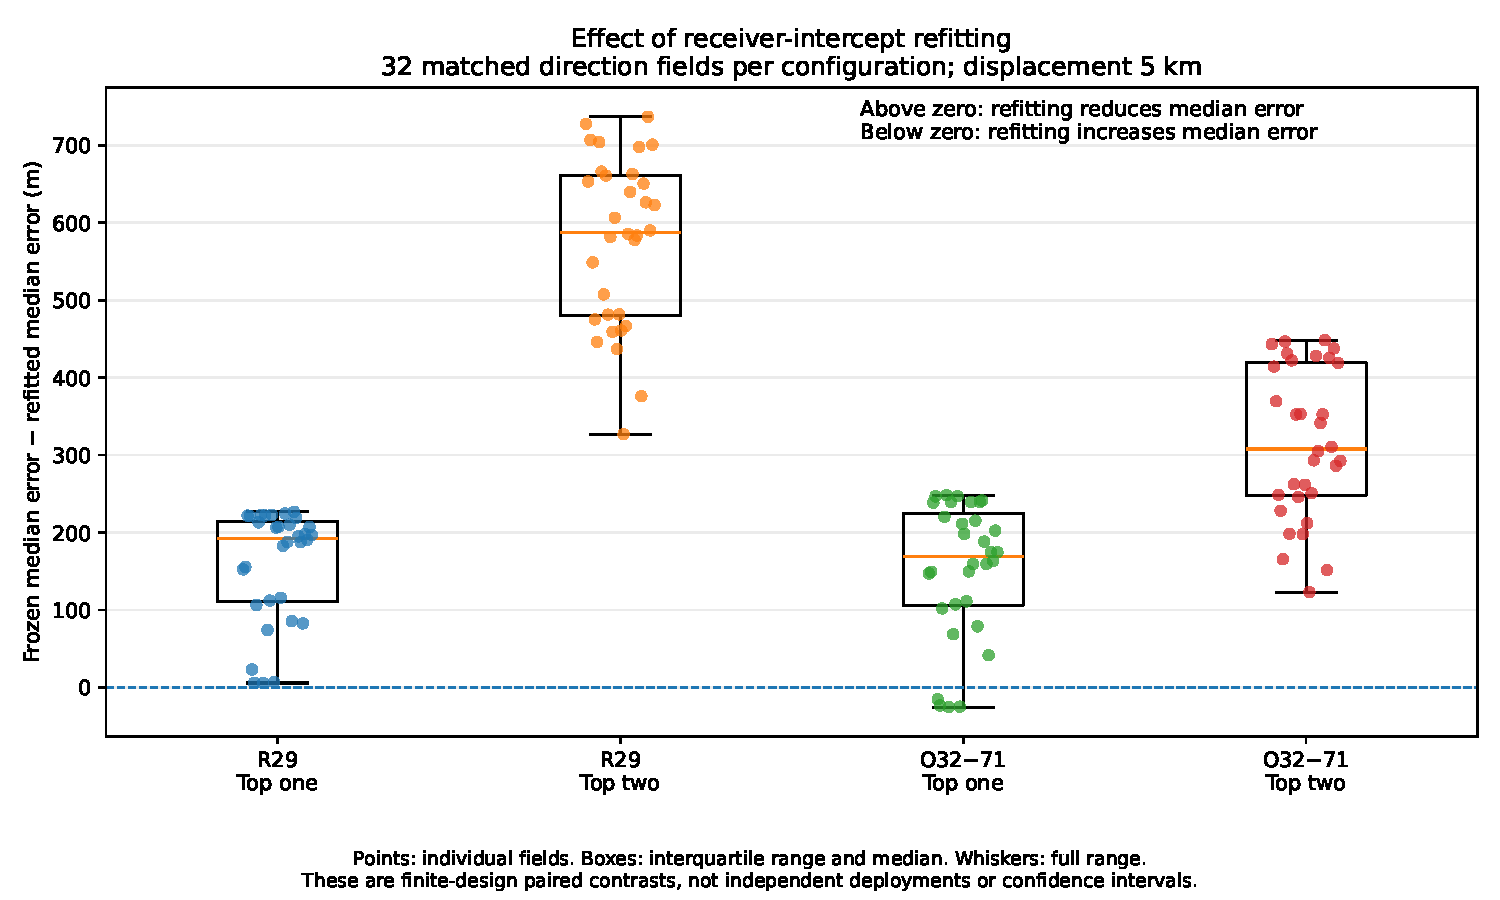
\includegraphics[width=\textwidth]{paired_calibration_32_fields.pdf}
\caption{Every field-level paired WCL contrast. Positive values favor refitting; the four negative O32$-$71 top-one cases are retained. Boxes show the median and interquartile range, whiskers the full range. These are specified directions within one deployment, not confidence intervals or independent replications.}\label{fig:paired}
\end{figure}

Protection is not uniform. O32$-$71 top-one draws 4, 5, 9 and 14 become approximately 15--25~m worse after refitting than after freezing. The same sign reversals persist in the fixed touched-message subset. A universal claim that refitting protects every direction is therefore contradicted by the experiment. The original two-field top-two R29 frozen result of $117.0\%$ remains valid for that smaller field set; $99.83\%$ is the expanded-set summary, not a correction that erases the earlier result.

In the top-two cells, the targets occur in 1845/2498 R29 messages and 1817/2498 O32$-$71 messages (73.9\% and 72.7\%). The small refit whole-population changes are consequently not explained solely by an untouched majority. Median paired benefits restricted to these fixed affected subsets are 740.37~m and 463.71~m, respectively. These are differences of subset medians, not a statement that every affected message improves. Untouched predictions are invariant in both arms.

The two configurations share the targeted BS14/BS69 coordinates, reference intercepts and calibration population. Other receiver coordinates, roster composition and evaluation identities differ. This tests behavior in two specified contexts; it does not isolate the cause of the four reversals or establish an independent second deployment.

\subsection{What Refitting Changes}\label{sec:weights}
With raw RSSI fixed, define $z_i=10^{-(A'_{0,i}-A_{0,i})/10}$. The unnormalized and normalized weights satisfy
\begin{equation}
 w'_i=w_i z_i,\qquad p'_i=\frac{p_i z_i}{\sum_j p_j z_j},\qquad p_i=\frac{w_i}{\sum_jw_j}.
\label{eq:weights}
\end{equation}
For the same perturbed coordinates, the prediction difference is
\begin{equation}
 \widehat{\mathbf x}_{\mathrm{refit}}-\widehat{\mathbf x}_{\mathrm{frozen}}
 =\sum_i(p'_i-p_i)\mathbf a'_i.
\label{eq:prediction}
\end{equation}
These are elementary consequences of the implemented WCL formula, not new theoretical claims. The saved weight and prediction checks verify the identities numerically. Refitting changes the weight assigned to a displaced receiver and the normalized weights of all selected receivers, even when non-target intercepts are unchanged. That provides a concrete mechanism for altered coordinate sensitivity without modifying the observations.

Downweighting does not guarantee a better estimate: the remaining geometry, observation/model error and the direction of the displaced contribution also matter. The four one-target reversals and the six existing signed-rotation refit/frozen pairs (Supplement S12.7) retain that boundary. Equations~\ref{eq:weights}--\ref{eq:prediction} do not decompose error magnitudes or population medians additively. The identified effect is the calibration-state intervention in this pipeline, not validation of the physical receiver map.

For the fixed set $H=\{q:G_q\cap T\ne\varnothing\}$ of messages selecting a target, define $b_{qr}=\sum_{i\in G_q\cap T}p_{qir}$ and $B=\operatorname{median}_r\operatorname{median}_{q\in H}b_{qr}$. Table~\ref{tab:weights} reports the normalized target-weight mass, not an unnormalized RSSI weight or a whole-population mean. Frozen weights are also the reference weights because the observations and intercepts are unchanged. Supplement S17.2 supplies receiver-specific intercept shifts and their ranges.

\begin{table}[htbp]\centering\small
\caption{Target-weight mass and error benefit in the fixed affected-message set $H$; 32 fields per cell. $B$ is the median across fields of the within-$H$ median normalized target-weight mass. $\Delta_H$ is the median across fields of frozen-minus-refitted error medians within $H$, not a median of individual-message differences. All populations contain 2498 messages.}\label{tab:weights}
\begin{tabular}{lrrrrr}
\toprule Configuration & $|H|$ & Frozen $B$ & Refitted $B$ & $\Delta_H$ (m) & $+/-$ fields\\\midrule
R29, $k=1$ & 1026 & 0.21824 & 0.00020675 & 618.66 & 32/0\\
R29, $k=2$ & 1845 & 0.21890 & 0.00015850 & 740.37 & 32/0\\
O32$-$71, $k=1$ & 1059 & 0.18468 & 0.00016776 & 492.21 & 28/4\\
O32$-$71, $k=2$ & 1817 & 0.12098 & 0.00008354 & 463.71 & 32/0\\
\bottomrule
\end{tabular}\end{table}


Across fields, median target-intercept increases are 31.30 dB for the one-target BS14 cell, and 31.11/34.19 dB for BS14/BS69 in the two-target cell on both configurations. The matching-target context explains this equality; it is not an independent second calibration. In the four adverse O32$-$71 one-target fields, within-$H$ median target weight still falls from 0.18468 to 0.000270--0.000287, yet the affected-subset frozen-minus-refitted error contrast is negative ($-38.53$ to $-40.83$ m). Thus downweighting is observed even in the counterexamples and does not itself guarantee accuracy.


\FloatBarrier
\subsection{Four-Pipeline Corruption-Load Context}\label{sec:load}
The four-pipeline load surface distinguishes the number of affected receivers from their displacement magnitude (Figure~\ref{fig:load}). Under map-specific refitting, one receiver displaced by 10~km produces across-method central changes between $-0.8\%$ and $+0.6\%$ on R29. Full-map corruption instead gives $+845.2\%$ for WCL, $+369.8\%$ for ABS, $+242.9\%$ for DIFF and $+582.9\%$ for Min-Max. O32$-$71 preserves this sparse--dense ordering, with respective full-roster changes of $+895.3\%$, $+399.4\%$, $+188.3\%$ and $+581.5\%$. These are finite-design median responses, not worst-case guarantees for an isolated receiver.

\begin{figure}[htbp]\centering
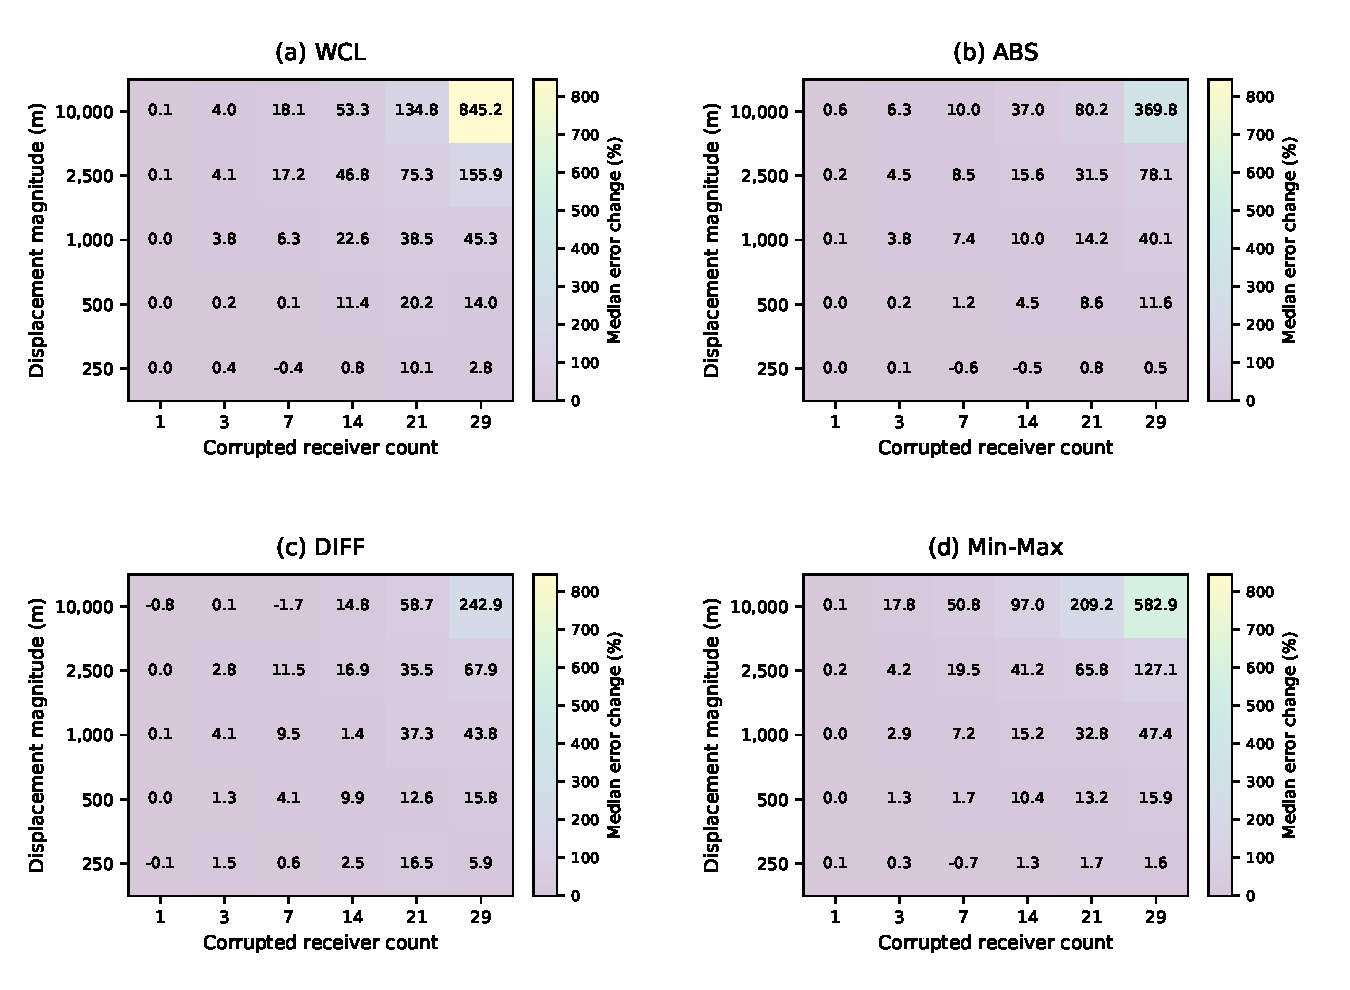
\includegraphics[width=\textwidth]{Fig1_Corruption_Load_Surface.pdf}
\caption{Four-pipeline corruption-load surface on R29. The five expansion magnitudes are shown; the historical 5-km slice remains in Supplement S16. Cells use eight target/direction fields except the 500-m slice, which uses 32. Signed annotations retain negative responses; Supplement S2/S14 supplies the percentages and absolute ranges.}\label{fig:load}
\end{figure}

Intermediate loads do not share a universal monotone response. Across eight reference constructions, exactly seven receivers displaced by 10~km yield positive central changes for WCL, ABS and Min-Max but DIFF changes between $-26.3\%$ and $-1.7\%$. This does not make corruption beneficial in general: errors in a fixed map and radio model can compensate in a particular objective. Large within-cell ranges also remain. For example, the 32-draw all-receiver 500-m WCL arm spans 510--903~m around a central 681~m. Corruption count and magnitude are useful descriptors, but they do not determine the observed outcome without the target, direction and pipeline conditions.


\FloatBarrier
\section{Receiver Participation and Affected Service Regions}\label{sec:participation}
\subsection{Identity Tracing beyond a Receiver-Count Threshold}\label{sec:identity}
Receiver participation is strongly nonuniform. Let $G_q$ be the raw-RSSI-selected reference receiver set for message $q$, and let $T_k$ contain the globally most-selected $k$ receivers. The selected-support exhaustion statistic is
\begin{equation}C(k)=\frac1N\sum_q\mathbf1\{G_q\subseteq T_k\}.\label{eq:exhaustion}\end{equation}
It counts messages retaining no selected uncorrupted receiver when all receivers in $T_k$ are displaced. It requires receiver identities and reception records, not localization-error outcomes or physical coordinate truth.

The receiver-window control traces a specific identity through a change in rank. In native O33 with BS71 substituted by its R29 coordinate, BS10 enters at rank seven with a ten-receiver window and rank six with a five-receiver window. The same 335 of 2495 messages become newly exhausted when BS10 enters. Among the two adjacent increases from $k=5$ to 6 and from $k=6$ to 7, the larger increase for WCL, ABS and DIFF moves with this event; Min-Max retains the larger increase from six to seven. That evidence links a transition to receiver participation and affected messages while retaining an architecture exception.

\begin{table}[htbp]\centering\small
\caption{O33-substituted window control at 5 km and $n=4.7$. Error increments are percentage-point differences between successive retained condition summaries, normalized by each method/window reference. New count denotes newly exhausted messages. The two BS10 rows contain the same 335 of 2495 messages. Cap ten uses eight fields per condition; cap five uses four. These are not paired same-vector changes across $k$.}\label{tab:o33window}
\begin{tabular}{rlrrrrrr}
\toprule Cap & Increment & Entering & New count & WCL & ABS & DIFF & Min-Max\\\midrule
10 & $5\to6$ & BS9 & 37 & +4.3 & +3.2 & +0.8 & +15.6\\
10 & $6\to7$ & BS10 & 335 & +129.6 & +62.4 & +40.7 & +107.8\\
5 & $5\to6$ & BS10 & 335 & +97.5 & +43.3 & +30.0 & +56.1\\
5 & $6\to7$ & BS32 & 107 & +52.8 & +20.1 & +3.5 & +65.1\\
\bottomrule
\end{tabular}\end{table}

The O33 comparison uses the unchanged 33-identity substituted map, not the raw catalogue BS71 coordinate. Conditions use independent uniform angles from NumPy \texttt{default\_rng} with seed $8800+k+101r$, consumed in ascending numeric target-ID order. The seed changes with $k$, and the cap-five field budget differs from cap ten; the increments therefore compare the retained condition summaries, not an isolated same-field effect of adding a receiver. Supplement S12.3 gives absolute errors, source precision and the identity check.
The broader R29 ranked curves in Figure~\ref{fig:rank} show the magnitude of the effect. At 5~km, the $k=6$ to $k=7$ central increments are 183.9, 26.8, 35.4 and 145.3 percentage points for WCL, ABS, DIFF and Min-Max. WCL's eight-field error ranges are 854--910~m at six and 1851--2322~m at seven. O32$-$71 also has positive increments for all four pipelines (111.3, 53.3, 36.9 and 93.3 points). Common-roster controls and the exponent checks preserve the positive directions while changing amplitudes.

\begin{figure}[htbp]\centering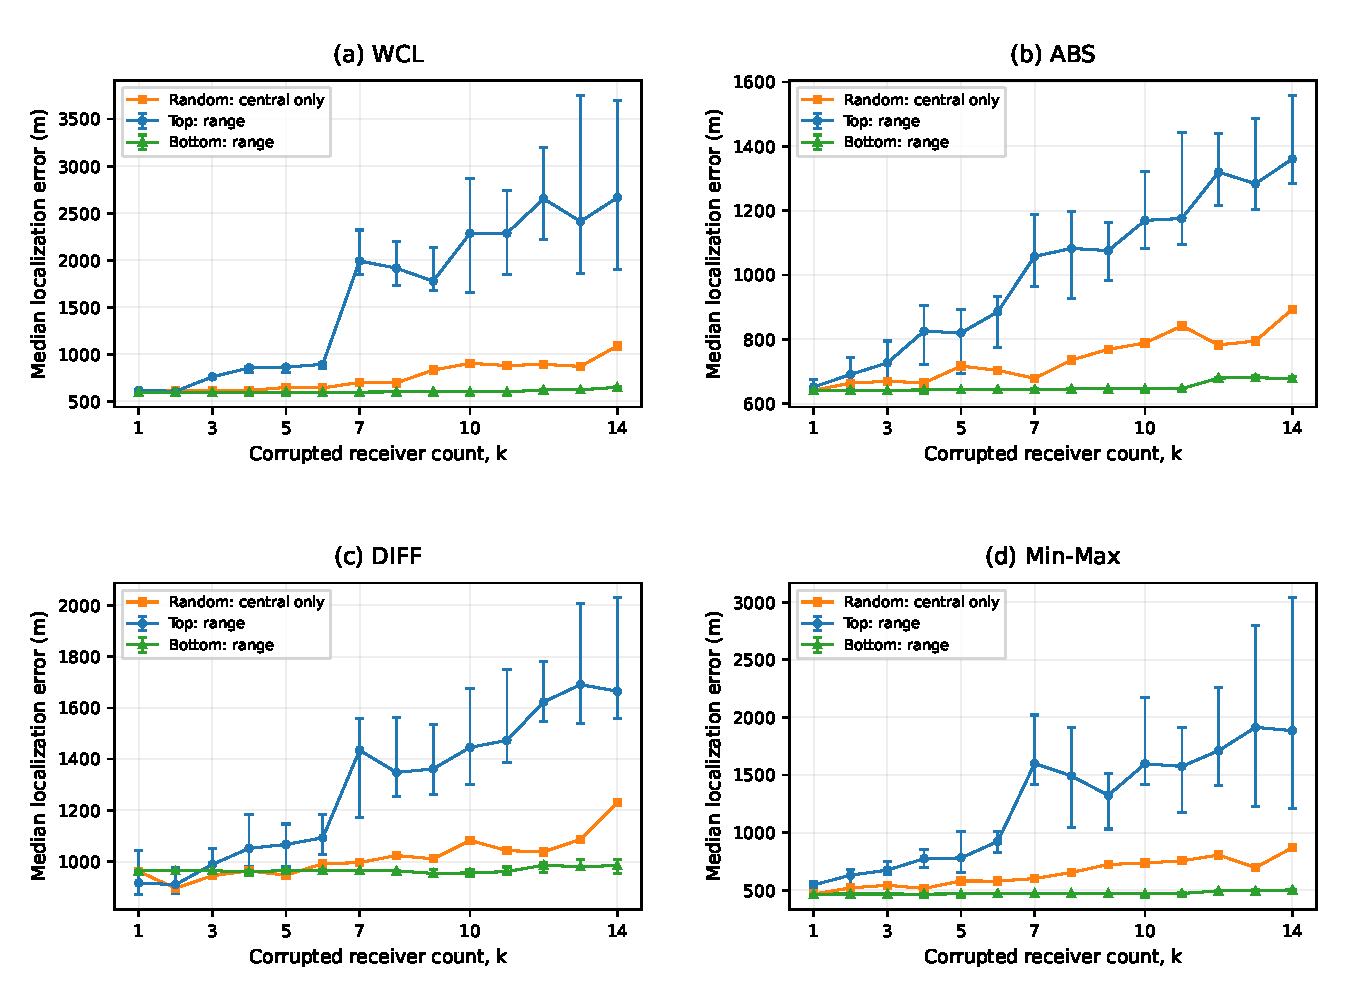
\includegraphics[width=\textwidth]{Fig2_Exposure_Topology.pdf}
\caption{R29 ranked-receiver corruption at 5~km. Top and bottom curves have eight direction fields; bars show full message-median ranges. The random curve retains its central summary only because its historical individual ranges were not preserved. Missing ranges are not reconstructed from the medians. All arms use map-specific recalibration.}\label{fig:rank}\end{figure}

On R29, $C(6)=5.6045\%$ and $C(7)=19.8159\%$: 355 messages are newly exhausted. The corresponding O32$-$71 count is 327, or 13.0905 percentage points. The top-seven identity set is stable under full-calibration and disjoint-half rankings. However, adding a receiver changes its coordinate influence as well as the support event, and the original top-$k$ direction seeds depend on $k$. The design does not independently manipulate exhaustion as the only cause of the error transition.

\subsection{Concentration and Dependence}\label{sec:geography}
The support event is geographically concentrated. At 500-m and 1-km cells, 354/355 newly exhausted R29 messages and 326/327 O32$-$71 messages occupy a single dominant cell. The primary R29 WCL field-first top-seven-minus-top-six contrast is approximately 1099~m; the direction-first message statistic used for cluster resampling is 1411.92~m. The order of medians differs, so these values are not conflicting estimates of the same statistic.

The 1-km spatial-cell intervals for that latter WCL statistic include zero on both maps ($-24.75$ to 2486.18~m on R29 and $-5.46$ to 1971.74~m on O32$-$71). The pre-specified spatial criterion G6 fails. Complete 5-, 15- and 30-minute time-block resampling yields positive intervals, but these are conditional on the realized direction fields and within-campaign block composition. They do not restore spatial generality or represent independent routes. The appropriate operational interpretation is a vulnerable service-region segment, not a spatially homogeneous risk law.

\begin{figure}[htbp]\centering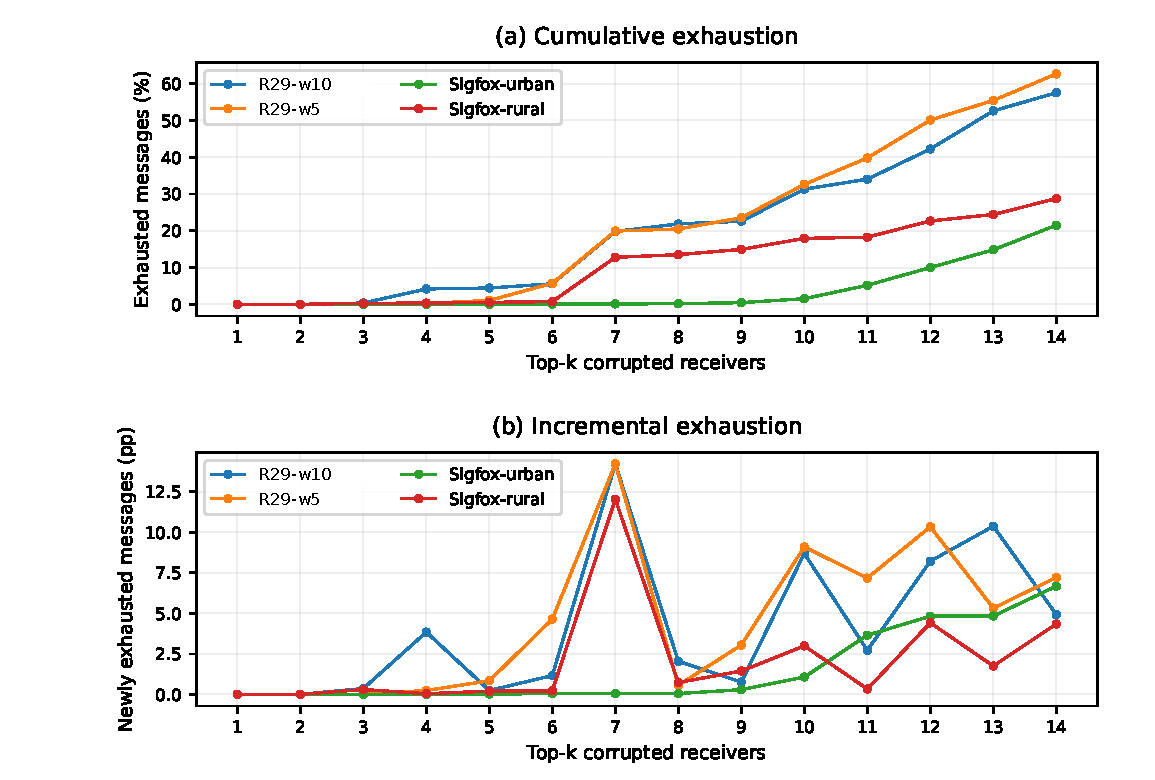
\includegraphics[width=0.90\textwidth]{Fig3_Selection_Set_Exhaustion_R29.pdf}
\caption{Selected-support exhaustion and its increments on R29 under the ten- and five-receiver windows (R29-w10/R29-w5), together with Sigfox structural controls. The R29 event remains at seven; this plot is not the O33-substituted migration tabulated separately. Rural Sigfox has an early concentrated event; urban Sigfox does not reproduce that integer threshold. Sigfox validates a data-side signature only, not localization performance.}\label{fig:exhaustion}\end{figure}
Rural Sigfox adds 2822 newly exhausted messages among 23,467 at $k=6$ to seven (12.025\%), whereas urban Sigfox adds six among 13,163 (0.0456\%). Figure~\ref{fig:exhaustion} therefore does not assert that a cliff occurs everywhere. It illustrates that the structural diagnostic responds to different participation patterns. Full counts, rank stability and conditional resampling outputs are retained in Supplement S4, S11--S13.

\subsection{Approximate Exposure Matching}\label{sec:bins}
The cumulative exposure share is $S(T)=\sum_q|G_q\cap T|/\sum_q|G_q|$, with denominator 10,680 selected receptions on R29. Eight subsets are retained in each bin centred at $S=0.10,\ldots,0.50$ with tolerance $\pm0.025$ and one 5-km field per subset. Exact share, subset size, identity and direction vary jointly. In the first bin, WCL effects range from 0.6\% to 46.2\%; in the last, 17.7\% to 136.5\%. These contrasts show that the tested binned descriptor does not tightly specify these outcomes, but do not isolate co-occurrence or rule out every predictive function of exact exposure. All 40 configurations and their recovered outputs remain in Supplement S3/S14 and the evidence package.

\section{Spatial Interventions and Reference-Frame Interpretation}\label{sec:spatial}
\subsection{Different Fields at the Same Displacement Scale}\label{sec:families}
At 5~km displacement of all R29 receivers, the eight-field isotropic median WCL degradation is 434.0\%, compared with 624.7\% for the specified coherent translation and 348.4\% for the specified inward field. ABS has a different ordering (148.2\%, 144.5\%, 172.2\%). These comparisons establish differences between the specified constructions, not a universal family ranking with equal directional replication.
\begin{figure}[htbp]\centering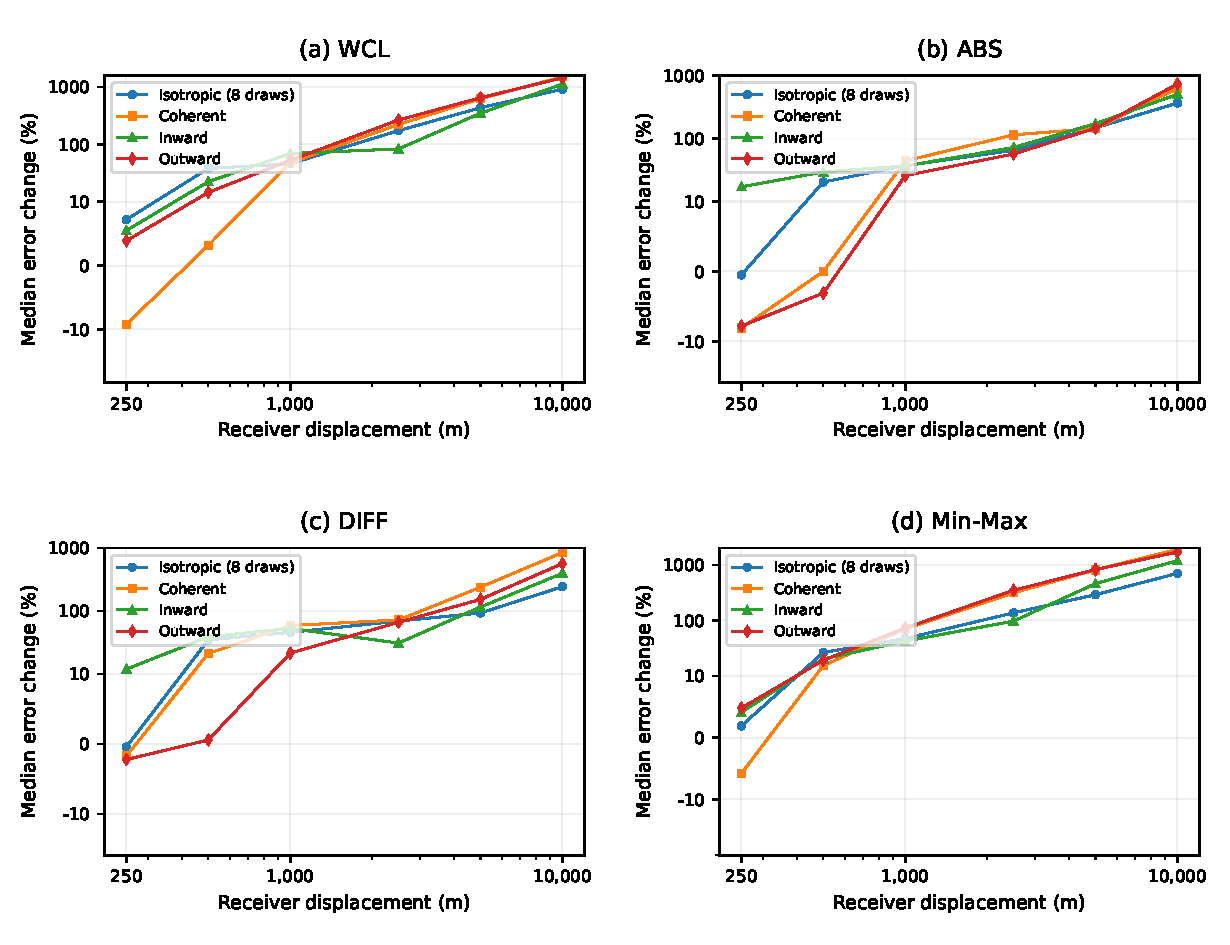
\includegraphics[width=\textwidth]{Fig5_Spatial_Error_Structure.pdf}
\caption{Spatial-family responses on R29. Isotropic values summarize eight fields; coherent, inward and outward entries each use one specified construction per magnitude. Inward displacement is unclipped and need not compress the map. The horizontal axis is logarithmic. The vertical axis is symmetric-logarithmic, with a linear interval from $-10\%$ to $+10\%$. The direction budget and operator are part of the comparison.}\label{fig:families}\end{figure}
The inward 5-km field moves 16 of 29 receivers through the transmitter centroid, and ten finish farther from it than initially. At 10~km, the corresponding counts are 22 and 16. A twelve-angle coherent sweep also exposes anisotropy: at 250~m, R29 WCL changes by $-9.7\%$ at $150^\circ$ but $+30.2\%$ at $330^\circ$. The observed preferred sector does not determine whether a relative frame discrepancy belongs to the receiver map, transmitter GPS, or another shared spatial bias.

\subsection{A Rotation Ordering That Does Not Transfer}\label{sec:rotation}
The original $+5^\circ$ R29 rotation about the unweighted receiver centroid gives $+49.8\%$ WCL degradation. Its four-field median-displacement-matched isotropic comparator gives $+22.7\%$, an excess of 27.1 points. Completing that comparator to eight fields gives $+19.9\%$, or 29.9 points. The pre-specified native O32$-$71 transfer reverses this ordering: rotation gives $+11.0\%$ against the eight-field isotropic median of $+14.9\%$. G4 therefore fails and remains failed.

Let $\mathbf c_u$ be the unweighted map centroid and $\mathbf c_o$ the operational centroid obtained by averaging reference-map normalized WCL predictions across evaluation messages. Reference intercepts are fitted on calibration data; evaluation transmitter coordinates and error outcomes do not enter $\mathbf c_o$. For rotation matrix $R$,
\begin{equation}
 \mathbf c_u+R(\mathbf a_i-\mathbf c_u)
 =\mathbf c_o+R(\mathbf a_i-\mathbf c_o)+(R-I)(\mathbf c_o-\mathbf c_u).
\label{eq:pivot}
\end{equation}
This exact coordinate identity identifies the translation associated with changing the pivot; it is not an additive decomposition of median localization errors. On R29, the centroids are 3359.2~m apart, producing a 293.0-m shift at $326.7^\circ$ under $+5^\circ$ rotation, near the adverse translation sector. The O32$-$71 shift is 137.5~m at $22.5^\circ$.

Post-failure controls rotate about $\mathbf c_o$ and randomize directions while preserving each receiver's exact rotation-induced displacement magnitude. Table~\ref{tab:rotation} and Figure~\ref{fig:rotation} display the individual-control context. R29's operational rotation lies inside its sampled isotropic range, with two controls worse; O32$-$71 lies above all eight controls. The positive median contrasts are useful descriptive results, not a universal eight-point penalty or a replacement confirmatory test.

\begin{table}[htbp]\centering\small
\caption{Five-degree WCL comparisons. Isotropic entries are medians and full ranges over eight fields. The contrast is rotation minus control median, normalized by the native reference. Operational/exact-profile rows are post-failure diagnostics.}\label{tab:rotation}
\begin{tabularx}{\textwidth}{llrrYr}
\toprule Construction & Map & Reference (m)&Rotation (m)&Isotropic median [range] (m)&Contrast (pp)\\\midrule
Legacy&R29&597.7&895.3&716.5 [537.9,895.6]&+29.91\\
Legacy&O32$-$71&593.7&659.1&682.4 [605.0,776.7]&$-3.93$\\
Operational/exact&R29&597.7&671.6&619.7 [554.0,692.6]&+8.68\\
Operational/exact&O32$-$71&593.7&627.1&577.9 [548.7,612.2]&+8.29\\\bottomrule
\end{tabularx}\end{table}
\begin{figure}[htbp]\centering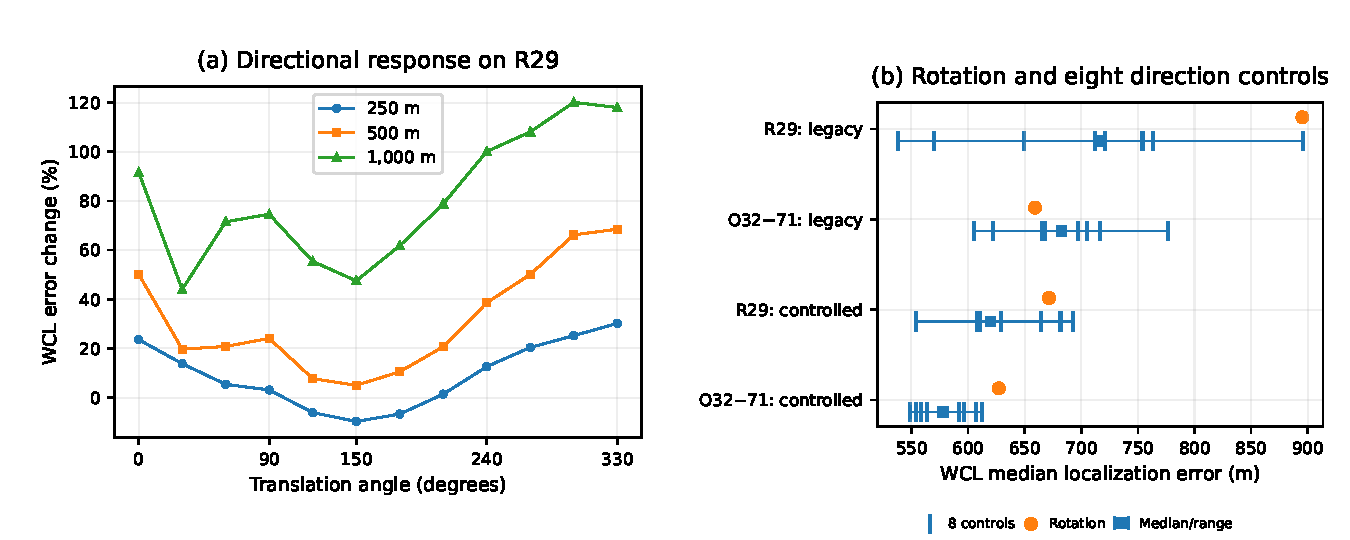
\includegraphics[width=\textwidth]{Fig6_Directional_and_Affine_Structure.pdf}
\caption{Directional response and full sampled rotation-control dispersion. Legacy and operational rows use different pivots and comparator definitions. The common-roster comparison remains separate from the native-map comparison; Supplement S12/S14 provides all methods and each control value.}\label{fig:rotation}\end{figure}

The native comparison changes roster, population and field geometry together. The R27/O27 common-roster WCL contrasts remain positive (25.22 and 7.94 points), showing different amplitude rather than an assignment-only sign reversal. BS71 is held at the recovered coordinate in both common-27 references. Exponent sensitivity preserves the native WCL sign reversal and the positive operational median contrasts at $n=3.5,4.7,6.0$, without eliminating sampled direction variability.

\subsection{Secondary Spatial and Mixed-Error Controls}\label{sec:secondary}
Uniform scaling by 0.98, 0.99, 1.01 or 1.02 gives small changes across the tested R29 implementations; WCL remains within approximately $\pm2\%$. Clustered corruption can have a much larger central WCL response than random corruption of the same count (115.5\% versus 8.9\% for seven receivers), but the eight-draw ranges overlap. The response depends strongly on which cluster is affected; the data do not establish population-level separation.

Adding 20-m ubiquitous jitter to sparse 5-km failures changes the retained mixed-minus-pure central summaries by approximately two percentage points or less. This describes one mixture, not linear superposition. The pooled top-six to top-seven WCL quantile changes are 1073~m at P50, 528~m at P90 and 312~m at P95. These are marginal summaries of four repeated evaluations of 2498 messages, not 9992 independent observations; they neither identify harmed-message subgroups nor show that most messages worsen. Complete values and the percentile figure appear in Supplement S7--S8 and S18. These controls characterize additional tested error fields and distributional summaries.

\section{Discussion and Limitations}\label{sec:discussion}
The matched WCL intervention demonstrates that the calibration state materially changes the measured median-error response to identical coordinate corruption. With recalibration available, the tested two-target fields produce small changes in aggregate error; with calibration frozen, the changes are much larger. These are different, legitimate operating conditions. Recalibration can improve accuracy under its stated information requirements, but the resulting low aggregate error does not validate the receiver map or establish robustness when adaptation is unavailable. The four adverse one-receiver fields show why the benefit must remain conditional.

The measured suppression is conditional on these unconstrained receiver-wise intercept fits and the exponential WCL weighting in Equation~\ref{eq:wcl}. It has not been established for bounded or regularized calibration, shared-intercept models, or a different weighting law. Coordinate-robustness comparisons should therefore report both the calibration constraints and the weighting rule.

Receiver participation provides a different kind of evidence. The same-identity window control links the location of a transition to a receiver and its message set, but it does not separately manipulate geometry and exhaustion. Its practical value is to identify concentrated dependence on a receiver set, followed by inspection of the affected service region. The failed spatial-cell criterion limits transportability to other service regions; the positive temporal intervals do not remove that spatial limitation.

The rotation analysis shows why transformation names must be accompanied by their construction. Changing a pivot changes the coordinate field; reference weights define an operational centroid particular to the pipeline and corpus. The exact coordinate identity clarifies that construction, while sampled comparisons characterize the observed error response. The failed transfer and direction-dependent comparisons support reference-specific interpretation.

\begin{table}[htbp]\centering\small
\caption{Practical interpretation and limits of the principal findings.}\label{tab:interpretation}
\begin{tabularx}{\textwidth}{YYY}\toprule Finding & Evaluation practice & Limit\\\midrule
Calibration-dependent sensitivity & Report the calibration state, intercept constraints and weighting law; compare matched refit/frozen states when adaptation is consequential. & WCL-specific intervention; finite directions; four adverse sparse cases; no proof of physical coordinate accuracy.\\
Participation-conditioned damage & Trace which messages select the affected receivers and where they occur, rather than reporting only corrupted count. & Association, not isolated exhaustion mediation; one concentrated route region and a Min-Max exception.\\
Reference/pivot-dependent spatial response & Specify map, roster, pivot, angle/directions and receiver-wise displacement profile alongside error magnitude. & Coordinate algebra is not additive error algebra; native maps differ; sampled ordering is not universal.\\\bottomrule\end{tabularx}
\end{table}
The empirical conditioning scheme $\Delta E_m=F_m(f,D,T,S,A\mid R)$ can summarize these inputs: load $f$, displacement $D$, participation $T$, spatial construction $S$, adaptation $A$ and reference configuration $R$. We do not estimate a universal function or identify its arguments as independent causal factors. Its role is experimental specification, not a newly fitted susceptibility predictor.

The principal limitations are substantive. All localization results concern one LoRaWAN deployment; Sigfox is a structural check only. Calibration and error scoring use released transmitter reference coordinates whose physical accuracy was not independently established. The within-campaign random split does not provide spatially or temporally independent validation, even after exact-content deduplication. R29's historical selection is incomplete and may use transmitter information, while catalogue coordinates are not surveyed truth. ABS/DIFF share a finite WCL-centred search, and the exponent is fixed in the primary programme. Original field budgets differ among experiment families. The 32-field extension increases direction coverage for one intervention but does not create independent deployments, resolve geographical concentration, establish all-estimator mechanisms or validate typical GNSS error magnitudes. Some historical arrays or ranges were not retained and are explicitly unavailable. New outputs are distinguished from saved historical records and from reporting reconstructions.

Shared source preparation is credited rather than counted as independent novelty. The source audit's primary centroid instrument uses raw RSSI, whereas the present WCL uses intercept-corrected RSSI; the audited current no-pair DIFF rule in that separate work differs from our all-pairs fallback. Equal method names or sample counts do not make results interchangeable. The reused identities and coordinate records accompany this article, so assessment does not depend on another manuscript's acceptance or headline conclusion.

\section{Conclusions}\label{sec:conclusion}
Matched comparisons demonstrate that receiver-intercept recalibration can substantially suppress the measured median-error response to severe receiver-coordinate corruption in the tested WCL pipeline. With the two highest-participation receivers displaced by 5~km, refitted changes of $+1.5\%$ and $-1.8\%$ contrast with frozen-state changes of $+99.8\%$ and $+50.2\%$ on the two specified configurations. All 32 two-target fields per configuration favor refitting; four one-target fields on O32$-$71 favor freezing. Quantified weight and affected-message diagnostics explain the calibration-state response while retaining those counterexamples.

The supporting analyses supply complementary evidence. The receiver-window comparison associates the local transition across $k=5$--7 with BS10 and the same selected-message set, without isolating support loss as the sole cause. The failed rotation transfer and change-of-pivot identity clarify reference-dependent spatial construction rather than a universal rotation penalty. The four-pipeline load surface establishes broader sparse--dense and architecture-dependent responses within the specified designs.

Measured coordinate robustness must therefore be reported together with the calibration opportunity, affected receiver/message sets and exact reference-frame construction. A small refitted median-error change is valid performance under adaptation, but cannot by itself establish map accuracy or the same response with calibration held fixed. The complete matched outcomes and diagnostics make that conditional finding inspectable and reproducible within the recorded campaign.

\section*{Supplementary Materials}
The Supplement retains all 39 original numerical tables and adds the complete paired-calibration record (S17) and the pooled-percentile profile (S18). The accompanying computational materials contain the unchanged baseline source/maps/results and the separately identified paired extension, its protocol, complete outputs and verification utilities. The source-version and claim-to-artifact indexes accompany the computational supplement.

\section*{Data and Code Availability}
The version-matched reproducibility package for this manuscript is version 1.1.0, identified by DOI \url{https://doi.org/10.5281/zenodo.23061691} \cite{baseline_archive} and maintained at \href{https://github.com/anantarj/receiver-coordinate-error-robustness-rssi-localization}{the GitHub repository}. It contains the complete 128-pair calibration intervention, numerical diagnostic tables, frozen baseline inputs and outputs, current document sources, and read-only verification utilities. The corresponding release asset is \path{PAPERB_SENSORS_EVIDENCE_v1.1.0_S8_300926.zip}. The preceding version 1.0.0 baseline remains available at \url{https://doi.org/10.5281/zenodo.22680802} and does not contain the 32-field extension. Original third-party measurements and the source catalogue are obtained separately from the fingerprinted public release. Author-created code is MIT-licensed; author-created documentation and derived non-code artifacts are CC BY 4.0, with third-party terms preserved. Saved-output verification, raw-input reconstruction and full experimental replay are distinguished in the supplied instructions.

\section*{Author Contributions}
Ananta Ranjan: conceptualization, methodology, software, validation, formal analysis, investigation, resources, data curation, writing---original draft, visualization, and project administration. Vijay Kumar Jha: supervision and writing---review and editing.

\section*{Funding}
No funding was received for this work.
\section*{Conflicts of Interest}
None of the authors have a conflict of interest to disclose.
\section*{Acknowledgment and AI-Assisted Tool Disclosure}
During this study and preparation of the manuscript, the authors used ChatGPT Sol 5.6 to assist with source-code inspection, code debugging, numerical consistency checks, analysis of computational outputs, and revision of the manuscript and supplementary material, and to assist with initial drafting and language revision. The authors directed these activities and repeatedly reviewed the AI-assisted work against the study's methods, computational records, and research objectives, checking implementation correctness and completeness and evaluating interpretations against the available evidence. The authors determined which suggestions to adopt, revise, or reject, made the final methodological and interpretive decisions, and take full responsibility for the manuscript and supplementary material.

\nocite{ref22}
\begingroup\small
\begin{thebibliography}{00}
\bibitem{ref1} K. W. K. Lui, W.-K. Ma, H. C. So, and F. K. W. Chan, "Semi-definite programming algorithms for sensor network node localization with uncertainties in anchor positions and/or propagation speed," IEEE Trans. Signal Process., vol. 57, no. 2, pp. 752-763, Feb. 2009, doi: 10.1109/TSP.2008.2007916.
\bibitem{ref2} G. Naddafzadeh-Shirazi, M. B. Shenouda, and L. Lampe, "Second order cone programming for sensor network localization with anchor position uncertainty," IEEE Trans. Wireless Commun., vol. 13, no. 2, pp. 749-763, Feb. 2014, doi: 10.1109/TWC.2013.120613.130170.
\bibitem{ref3} M. Angjelichinoski, D. Denkovski, V. Atanasovski, and L. Gavrilovska, "SPEAR: Source position estimation for anchor position uncertainty reduction," IEEE Commun. Lett., vol. 18, no. 4, pp. 560-563, Apr. 2014, doi: 10.1109/LCOMM.2014.020414.132780.
\bibitem{ref4} H. Lohrasbipeydeh, T. A. Gulliver, and H. Amindavar, "Unknown transmit power RSSD based source localization with sensor position uncertainty," IEEE Trans. Commun., vol. 63, no. 5, pp. 1784-1797, May 2015, doi: 10.1109/TCOMM.2015.2410300.
\bibitem{ref5} D. Denkovski, M. Angjelichinoski, V. Atanasovski, and L. Gavrilovska, "Geometric interpretation of theoretical bounds for RSS-based source localization with uncertain anchor positions," Digit. Signal Process., vol. 68, pp. 167-181, Sep. 2017, doi: 10.1016/j.dsp.2017.06.003.
\bibitem{ref6} V. Kumar, R. Arablouei, F. de Hoog, R. Jurdak, B. Kusy, and N. W. Bergmann, "Pseudo-linear localization using perturbed RSSI measurements and inaccurate anchor positions," Pervasive Mobile Comput., vol. 52, pp. 46-59, Jan. 2019, doi: 10.1016/j.pmcj.2018.11.004.
\bibitem{ref7} V. Kumar and R. Arablouei, "Self-localization of IoT devices using noisy anchor positions and RSSI measurements," Wireless Pers. Commun., vol. 124, no. 2, pp. 1623-1644, May 2022, doi: 10.1007/s11277-021-09423-x.
\bibitem{ref8} Y. Liu, G. Han, Y. Wang, Z. Xue, J. Chen, and C. Liu, "Received signal strength-based wireless source localization with inaccurate anchor positions," IEEE Sensors J., vol. 22, no. 23, pp. 23539-23551, Dec. 2022, doi: 10.1109/JSEN.2022.3213373.
\bibitem{ref9} Q. Wang and X. Li, "Source localization using RSS measurements with sensor position uncertainty," Int. J. Distrib. Sensor Netw., vol. 2023, Art. no. 9274297, 2023, doi: 10.1155/2023/9274297.
\bibitem{ref10} Y. Li, B. Mukhopadhyay, J. Xu, and M.-S. Alouini, "Experimental validation of cooperative RSS-based localization with unknown transmit power, path loss exponent, and precise anchor location," IEEE Trans. Wireless Commun., vol. 23, no. 11, pp. 16482-16497, Nov. 2024, doi: 10.1109/TWC.2024.3441643.
\bibitem{ref11} Q. Yan, Z. Luo, H.-M. Wang, B. Wang, and C. Gao, "An impulsive noise-resistant target localization approach with unknown model parameter learning," IEEE Internet Things J., vol. 12, no. 6, pp. 7421-7433, Mar. 2025, doi: 10.1109/JIOT.2024.3494870.
\bibitem{ref12} E. Gur and S. Sabach, "Fast and convergent method for large-scale sensor network localization with anchor uncertainty," ACM Trans. Sensor Netw., vol. 21, no. 5, Art. no. 49, pp. 1-30, 2025, doi: 10.1145/3757744.
\bibitem{ref13} M. Angjelichinoski, D. Denkovski, V. Atanasovski, and L. Gavrilovska, "Cramer-Rao lower bounds of RSS-based localization with anchor position uncertainty," IEEE Trans. Inf. Theory, vol. 61, no. 5, pp. 2807-2834, May 2015, doi: 10.1109/TIT.2015.2409270.
\bibitem{ref14} X. Mei, H. Wu, J. Xian, X. Chen, and Y. Zang, "Theoretical analysis of hybrid RSS and TOA localization with stratified propagation under inaccurate anchors in UAIoTs," Intell. Mar. Technol. Syst., vol. 4, Art. no. 2, 2026, doi: 10.1007/s44295-025-00085-0.
\bibitem{ref15} A. Ranjan, ``Published, Unjoined: Coordinate Provenance and Reception Support in a Public LPWAN Localization Benchmark,'' unpublished manuscript, revision R5.1, 6 September 2026.
\bibitem{ref16} J. N. Ash and R. L. Moses, "On the relative and absolute positioning errors in self-localization systems," IEEE Trans. Signal Process., vol. 56, no. 11, pp. 5668-5679, Nov. 2008, doi: 10.1109/TSP.2008.927072.
\bibitem{ref17} A. A. Ababneh, "Knapsack-based sensor selection for target localization under energy and error constraints," IEEE Sensors J., vol. 21, no. 23, pp. 27208-27217, Dec. 2021, doi: 10.1109/JSEN.2021.3123734.
\bibitem{ref18} Y. Long, Y. Zeng, X. Xu, and Y. Huang, "Environment-aware wireless localization enabled by channel knowledge map," in Proc. IEEE Global Commun. Conf. (GLOBECOM), 2022, pp. 5354-5359, doi: 10.1109/GLOBECOM48099.2022.10001045.
\bibitem{ref19} M. Aernouts, R. Berkvens, K. Van Vlaenderen, and M. Weyn, "Sigfox and LoRaWAN datasets for fingerprint localization in large urban and rural areas," version 1.3, Zenodo, Jul. 19, 2019, doi: 10.5281/zenodo.3904158.
\bibitem{ref20} M. Aernouts, R. Berkvens, K. Van Vlaenderen, and M. Weyn, "Sigfox and LoRaWAN datasets for fingerprint localization in large urban and rural areas," Data, vol. 3, no. 2, Art. no. 13, 2018, doi: 10.3390/data3020013.
\bibitem{ref21} T. Janssen, R. Berkvens, and M. Weyn, "Benchmarking RSS-based localization algorithms with LoRaWAN," Internet Things, vol. 11, Art. no. 100235, Sep. 2020, doi: 10.1016/j.iot.2020.100235.
\bibitem{ref22} OpenAI, "ChatGPT (GPT-5.6 Sol)," 2026. [Online]. Available: https://chatgpt.com. Accessed: Sep. 5, 2026.
\bibitem{ref23} A. Ranjan, ``Pricing the Common-Mode Guarantee of a Pairwise-Differential RSSI Objective on a Public LPWAN Deployment,'' related letter manuscript, version dated Aug. 26, 2026.
\bibitem{baseline_archive} Ranjan, A.; Jha, V.K. Recalibration Can Mask Measured Sensitivity to Receiver-Coordinate Errors in RSSI Localization: reproducibility package, version 1.1.0, 2026. Zenodo. \url{https://doi.org/10.5281/zenodo.23061691}. Version-matched computational archive; the preceding version 1.0.0 baseline remains at \url{https://doi.org/10.5281/zenodo.22680802}.
\end{thebibliography}
\section*{Author Biographies}
\noindent\textbf{Ananta Ranjan} is pursuing the Ph.D. degree in computer science and engineering with the Department of Computer Science and Engineering, Birla Institute of Technology, Mesra, Ranchi, India. Research interests include wireless localization, low-power wide-area networks, Internet-of-Things measurement methodology, and reproducible experimental evaluation. ORCID: \url{https://orcid.org/0000-0002-1105-0666}.

\noindent\textbf{Vijay Kumar Jha} is a Professor with the Department of Computer Science and Engineering, Birla Institute of Technology, Mesra, Ranchi, India. Research interests include network security, big-data analytics, and data mining. ORCID: \url{https://orcid.org/0000-0001-7310-1177}.

\endgroup
\end{document}
